\begin{figure}[t]
\centering
\definecolor{vanRed}{HTML}{C5635F}
\definecolor{r2sGreen}{HTML}{2EB58F}
\scriptsize
\makebox[\linewidth][c]{\textbf{ALFWorld}}\\[1pt]
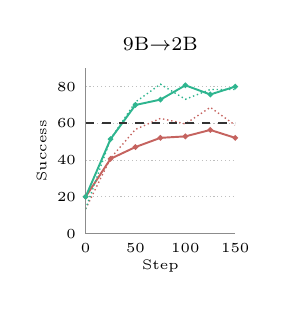
\begin{tikzpicture}
\begin{axis}[
  width=1.9cm, height=2.1cm, scale only axis,
  xmin=0, xmax=150, ymin=0, ymax=90, xtick={0,50,100,150}, ylabel={Success}, xlabel={Step},
  axis lines*=left, axis line style={black!45}, tick style={draw=none}, ytick pos=left,
  ymajorgrids, grid style={densely dotted, black!25}, every tick label/.append style={font=\tiny},
  ylabel style={font=\tiny, yshift=-3pt}, xlabel style={font=\tiny, yshift=4pt}, title style={font=\scriptsize, yshift=-3pt},
  title={9B$\to$2B},
]
\addplot[vanRed, line width=0.7pt, mark=*, mark size=0.6pt] coordinates {(0,20.0) (25,40.7) (50,47.1) (75,52.1) (100,52.9) (125,56.4) (150,52.1)};
\addplot[vanRed, densely dotted, line width=0.5pt] coordinates {(0,13.4) (25,41.0) (50,56.7) (75,62.7) (100,59.7) (125,68.7) (150,59.0)};
\addplot[r2sGreen, line width=0.7pt, mark=*, mark size=0.6pt] coordinates {(0,20.0) (25,51.4) (50,70.0) (75,72.9) (100,80.7) (125,75.7) (150,80.0)};
\addplot[r2sGreen, densely dotted, line width=0.5pt] coordinates {(0,13.4) (25,51.5) (50,71.6) (75,81.3) (100,73.1) (125,78.4) (150,78.4)};
\draw[dashed, black!80, line width=0.6pt] (rel axis cs:0,0.6693) -- (rel axis cs:1,0.6693);
\end{axis}
\end{tikzpicture}
\hfill
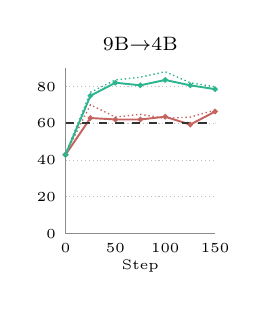
\begin{tikzpicture}
\begin{axis}[
  width=1.9cm, height=2.1cm, scale only axis,
  xmin=0, xmax=150, ymin=0, ymax=90, xtick={0,50,100,150},  xlabel={Step},
  axis lines*=left, axis line style={black!45}, tick style={draw=none}, ytick pos=left,
  ymajorgrids, grid style={densely dotted, black!25}, every tick label/.append style={font=\tiny},
  ylabel style={font=\tiny, yshift=-3pt}, xlabel style={font=\tiny, yshift=4pt}, title style={font=\scriptsize, yshift=-3pt},
  title={9B$\to$4B},
]
\addplot[vanRed, line width=0.7pt, mark=*, mark size=0.6pt] coordinates {(0,42.9) (25,62.9) (50,62.1) (75,62.1) (100,63.6) (125,59.3) (150,66.4)};
\addplot[vanRed, densely dotted, line width=0.5pt] coordinates {(0,43.3) (25,70.1) (50,63.4) (75,64.9) (100,62.7) (125,63.4) (150,67.2)};
\addplot[r2sGreen, line width=0.7pt, mark=*, mark size=0.6pt] coordinates {(0,42.9) (25,75.0) (50,82.1) (75,80.7) (100,83.6) (125,80.7) (150,78.6)};
\addplot[r2sGreen, densely dotted, line width=0.5pt] coordinates {(0,43.3) (25,76.9) (50,83.6) (75,85.1) (100,88.1) (125,82.1) (150,79.9)};
\draw[dashed, black!80, line width=0.6pt] (rel axis cs:0,0.6693) -- (rel axis cs:1,0.6693);
\end{axis}
\end{tikzpicture}
\hfill
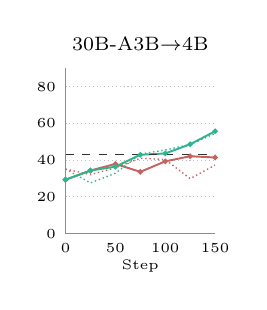
\begin{tikzpicture}
\begin{axis}[
  width=1.9cm, height=2.1cm, scale only axis,
  xmin=0, xmax=150, ymin=0, ymax=90, xtick={0,50,100,150},  xlabel={Step},
  axis lines*=left, axis line style={black!45}, tick style={draw=none}, ytick pos=left,
  ymajorgrids, grid style={densely dotted, black!25}, every tick label/.append style={font=\tiny},
  ylabel style={font=\tiny, yshift=-3pt}, xlabel style={font=\tiny, yshift=4pt}, title style={font=\scriptsize, yshift=-3pt},
  title={30B-A3B$\to$4B},
]
\addplot[vanRed, line width=0.7pt, mark=*, mark size=0.6pt] coordinates {(0,29.3) (25,34.3) (50,37.9) (75,33.6) (100,39.3) (125,42.1) (150,41.4)};
\addplot[vanRed, densely dotted, line width=0.5pt] coordinates {(0,35.1) (25,32.1) (50,35.8) (75,41.0) (100,40.3) (125,29.9) (150,37.3)};
\addplot[r2sGreen, line width=0.7pt, mark=*, mark size=0.6pt] coordinates {(0,29.3) (25,34.3) (50,36.4) (75,42.9) (100,43.6) (125,48.6) (150,55.7)};
\addplot[r2sGreen, densely dotted, line width=0.5pt] coordinates {(0,35.1) (25,27.6) (50,32.8) (75,43.3) (100,45.5) (125,48.5) (150,54.5)};
\draw[dashed, black!80, line width=0.6pt] (rel axis cs:0,0.4788) -- (rel axis cs:1,0.4788);
\end{axis}
\end{tikzpicture}
\hfill
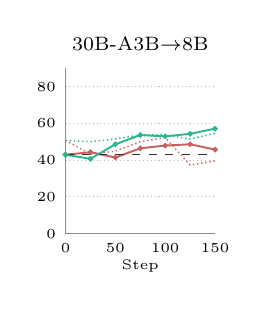
\begin{tikzpicture}
\begin{axis}[
  width=1.9cm, height=2.1cm, scale only axis,
  xmin=0, xmax=150, ymin=0, ymax=90, xtick={0,50,100,150},  xlabel={Step},
  axis lines*=left, axis line style={black!45}, tick style={draw=none}, ytick pos=left,
  ymajorgrids, grid style={densely dotted, black!25}, every tick label/.append style={font=\tiny},
  ylabel style={font=\tiny, yshift=-3pt}, xlabel style={font=\tiny, yshift=4pt}, title style={font=\scriptsize, yshift=-3pt},
  title={30B-A3B$\to$8B},
]
\addplot[vanRed, line width=0.7pt, mark=*, mark size=0.6pt] coordinates {(0,42.9) (25,44.3) (50,41.4) (75,46.4) (100,47.9) (125,48.6) (150,45.7)};
\addplot[vanRed, densely dotted, line width=0.5pt] coordinates {(0,50.7) (25,43.3) (50,44.8) (75,50.0) (100,52.2) (125,37.3) (150,39.6)};
\addplot[r2sGreen, line width=0.7pt, mark=*, mark size=0.6pt] coordinates {(0,42.9) (25,40.7) (50,48.6) (75,53.6) (100,52.9) (125,54.3) (150,57.1)};
\addplot[r2sGreen, densely dotted, line width=0.5pt] coordinates {(0,50.7) (25,50.0) (50,51.5) (75,53.7) (100,53.7) (125,51.5) (150,54.5)};
\draw[dashed, black!80, line width=0.6pt] (rel axis cs:0,0.4788) -- (rel axis cs:1,0.4788);
\end{axis}
\end{tikzpicture}
\hfill
\\[3pt]
\makebox[\linewidth][c]{\textbf{WebShop}}\\[1pt]
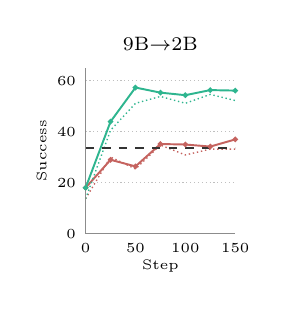
\begin{tikzpicture}
\begin{axis}[
  width=1.9cm, height=2.1cm, scale only axis,
  xmin=0, xmax=150, ymin=0, ymax=65, xtick={0,50,100,150}, ylabel={Success}, xlabel={Step},
  axis lines*=left, axis line style={black!45}, tick style={draw=none}, ytick pos=left,
  ymajorgrids, grid style={densely dotted, black!25}, every tick label/.append style={font=\tiny},
  ylabel style={font=\tiny, yshift=-3pt}, xlabel style={font=\tiny, yshift=4pt}, title style={font=\scriptsize, yshift=-3pt},
  title={9B$\to$2B},
]
\addplot[vanRed, line width=0.7pt, mark=*, mark size=0.6pt] coordinates {(0,18.0) (25,29.0) (50,26.4) (75,35.2) (100,35.0) (125,34.2) (150,37.0)};
\addplot[vanRed, densely dotted, line width=0.5pt] coordinates {(0,13.7) (25,30.1) (50,25.4) (75,34.8) (100,30.9) (125,33.2) (150,33.2)};
\addplot[r2sGreen, line width=0.7pt, mark=*, mark size=0.6pt] coordinates {(0,18.0) (25,44.0) (50,57.4) (75,55.4) (100,54.4) (125,56.4) (150,56.2)};
\addplot[r2sGreen, densely dotted, line width=0.5pt] coordinates {(0,13.7) (25,40.6) (50,51.2) (75,53.9) (100,51.2) (125,54.7) (150,52.3)};
\draw[dashed, black!80, line width=0.6pt] (rel axis cs:0,0.5159) -- (rel axis cs:1,0.5159);
\end{axis}
\end{tikzpicture}
\hfill
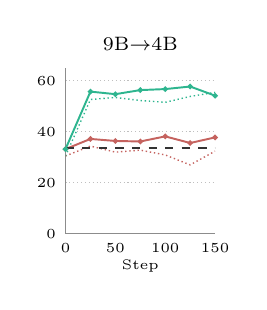
\begin{tikzpicture}
\begin{axis}[
  width=1.9cm, height=2.1cm, scale only axis,
  xmin=0, xmax=150, ymin=0, ymax=65, xtick={0,50,100,150},  xlabel={Step},
  axis lines*=left, axis line style={black!45}, tick style={draw=none}, ytick pos=left,
  ymajorgrids, grid style={densely dotted, black!25}, every tick label/.append style={font=\tiny},
  ylabel style={font=\tiny, yshift=-3pt}, xlabel style={font=\tiny, yshift=4pt}, title style={font=\scriptsize, yshift=-3pt},
  title={9B$\to$4B},
]
\addplot[vanRed, line width=0.7pt, mark=*, mark size=0.6pt] coordinates {(0,33.2) (25,37.2) (50,36.4) (75,36.2) (100,38.2) (125,35.6) (150,37.8)};
\addplot[vanRed, densely dotted, line width=0.5pt] coordinates {(0,30.5) (25,34.4) (50,32.0) (75,32.8) (100,30.9) (125,27.0) (150,32.4)};
\addplot[r2sGreen, line width=0.7pt, mark=*, mark size=0.6pt] coordinates {(0,33.2) (25,55.8) (50,54.8) (75,56.4) (100,56.8) (125,57.8) (150,54.2)};
\addplot[r2sGreen, densely dotted, line width=0.5pt] coordinates {(0,30.5) (25,52.7) (50,53.5) (75,52.3) (100,51.6) (125,53.9) (150,55.5)};
\draw[dashed, black!80, line width=0.6pt] (rel axis cs:0,0.5159) -- (rel axis cs:1,0.5159);
\end{axis}
\end{tikzpicture}
\hfill
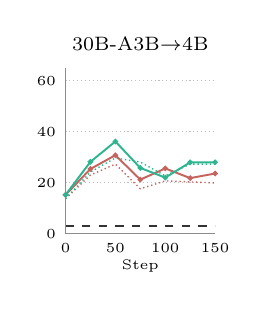
\begin{tikzpicture}
\begin{axis}[
  width=1.9cm, height=2.1cm, scale only axis,
  xmin=0, xmax=150, ymin=0, ymax=65, xtick={0,50,100,150},  xlabel={Step},
  axis lines*=left, axis line style={black!45}, tick style={draw=none}, ytick pos=left,
  ymajorgrids, grid style={densely dotted, black!25}, every tick label/.append style={font=\tiny},
  ylabel style={font=\tiny, yshift=-3pt}, xlabel style={font=\tiny, yshift=4pt}, title style={font=\scriptsize, yshift=-3pt},
  title={30B-A3B$\to$4B},
]
\addplot[vanRed, line width=0.7pt, mark=*, mark size=0.6pt] coordinates {(0,15.2) (25,25.4) (50,30.8) (75,21.2) (100,25.6) (125,21.8) (150,23.6)};
\addplot[vanRed, densely dotted, line width=0.5pt] coordinates {(0,13.7) (25,23.0) (50,27.3) (75,17.6) (100,20.7) (125,20.3) (150,19.9)};
\addplot[r2sGreen, line width=0.7pt, mark=*, mark size=0.6pt] coordinates {(0,15.2) (25,28.2) (50,36.2) (75,25.8) (100,22.0) (125,28.0) (150,28.0)};
\addplot[r2sGreen, densely dotted, line width=0.5pt] coordinates {(0,13.7) (25,24.2) (50,29.7) (75,28.1) (100,22.7) (125,27.3) (150,27.3)};
\draw[dashed, black!80, line width=0.6pt] (rel axis cs:0,0.0441) -- (rel axis cs:1,0.0441);
\end{axis}
\end{tikzpicture}
\hfill
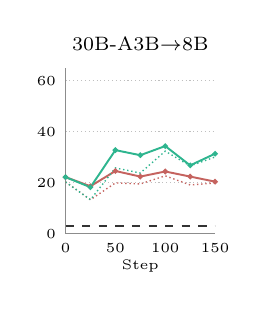
\begin{tikzpicture}
\begin{axis}[
  width=1.9cm, height=2.1cm, scale only axis,
  xmin=0, xmax=150, ymin=0, ymax=65, xtick={0,50,100,150},  xlabel={Step},
  axis lines*=left, axis line style={black!45}, tick style={draw=none}, ytick pos=left,
  ymajorgrids, grid style={densely dotted, black!25}, every tick label/.append style={font=\tiny},
  ylabel style={font=\tiny, yshift=-3pt}, xlabel style={font=\tiny, yshift=4pt}, title style={font=\scriptsize, yshift=-3pt},
  title={30B-A3B$\to$8B},
]
\addplot[vanRed, line width=0.7pt, mark=*, mark size=0.6pt] coordinates {(0,22.2) (25,18.6) (50,24.6) (75,22.4) (100,24.4) (125,22.4) (150,20.4)};
\addplot[vanRed, densely dotted, line width=0.5pt] coordinates {(0,20.3) (25,13.3) (50,19.9) (75,19.5) (100,22.7) (125,19.1) (150,19.9)};
\addplot[r2sGreen, line width=0.7pt, mark=*, mark size=0.6pt] coordinates {(0,22.2) (25,18.2) (50,32.8) (75,30.8) (100,34.4) (125,26.8) (150,31.4)};
\addplot[r2sGreen, densely dotted, line width=0.5pt] coordinates {(0,20.3) (25,13.3) (50,25.8) (75,23.8) (100,32.4) (125,26.6) (150,30.1)};
\draw[dashed, black!80, line width=0.6pt] (rel axis cs:0,0.0441) -- (rel axis cs:1,0.0441);
\end{axis}
\end{tikzpicture}
\hfill
\\[3pt]
\makebox[\linewidth][c]{\textbf{ScienceWorld}}\\[1pt]
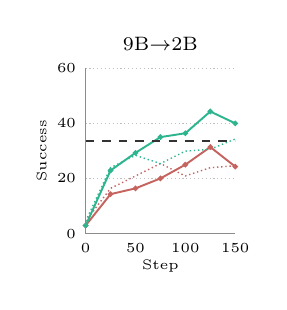
\begin{tikzpicture}
\begin{axis}[
  width=1.9cm, height=2.1cm, scale only axis,
  xmin=0, xmax=150, ymin=0, ymax=60, xtick={0,50,100,150}, ylabel={Success}, xlabel={Step},
  axis lines*=left, axis line style={black!45}, tick style={draw=none}, ytick pos=left,
  ymajorgrids, grid style={densely dotted, black!25}, every tick label/.append style={font=\tiny},
  ylabel style={font=\tiny, yshift=-3pt}, xlabel style={font=\tiny, yshift=4pt}, title style={font=\scriptsize, yshift=-3pt},
  title={9B$\to$2B},
]
\addplot[vanRed, line width=0.7pt, mark=*, mark size=0.6pt] coordinates {(0,2.9) (25,14.3) (50,16.4) (75,20.0) (100,25.0) (125,31.4) (150,24.3)};
\addplot[vanRed, densely dotted, line width=0.5pt] coordinates {(0,4.5) (25,16.4) (50,20.9) (75,25.4) (100,20.9) (125,23.9) (150,24.6)};
\addplot[r2sGreen, line width=0.7pt, mark=*, mark size=0.6pt] coordinates {(0,2.9) (25,22.9) (50,29.3) (75,35.0) (100,36.4) (125,44.3) (150,40.0)};
\addplot[r2sGreen, densely dotted, line width=0.5pt] coordinates {(0,4.5) (25,23.9) (50,28.4) (75,25.4) (100,29.9) (125,30.6) (150,34.3)};
\draw[dashed, black!80, line width=0.6pt] (rel axis cs:0,0.5595) -- (rel axis cs:1,0.5595);
\end{axis}
\end{tikzpicture}
\hfill
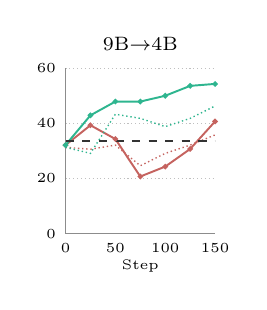
\begin{tikzpicture}
\begin{axis}[
  width=1.9cm, height=2.1cm, scale only axis,
  xmin=0, xmax=150, ymin=0, ymax=60, xtick={0,50,100,150},  xlabel={Step},
  axis lines*=left, axis line style={black!45}, tick style={draw=none}, ytick pos=left,
  ymajorgrids, grid style={densely dotted, black!25}, every tick label/.append style={font=\tiny},
  ylabel style={font=\tiny, yshift=-3pt}, xlabel style={font=\tiny, yshift=4pt}, title style={font=\scriptsize, yshift=-3pt},
  title={9B$\to$4B},
]
\addplot[vanRed, line width=0.7pt, mark=*, mark size=0.6pt] coordinates {(0,32.1) (25,39.3) (50,34.3) (75,20.7) (100,24.3) (125,30.7) (150,40.7)};
\addplot[vanRed, densely dotted, line width=0.5pt] coordinates {(0,31.3) (25,30.6) (50,32.1) (75,24.6) (100,29.1) (125,32.1) (150,35.8)};
\addplot[r2sGreen, line width=0.7pt, mark=*, mark size=0.6pt] coordinates {(0,32.1) (25,42.9) (50,47.9) (75,47.9) (100,50.0) (125,53.6) (150,54.3)};
\addplot[r2sGreen, densely dotted, line width=0.5pt] coordinates {(0,31.3) (25,29.1) (50,43.3) (75,41.8) (100,38.8) (125,41.8) (150,46.3)};
\draw[dashed, black!80, line width=0.6pt] (rel axis cs:0,0.5595) -- (rel axis cs:1,0.5595);
\end{axis}
\end{tikzpicture}
\hfill
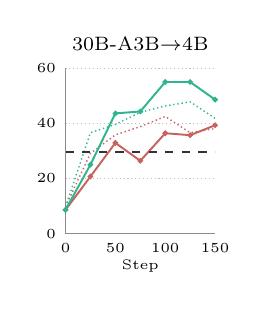
\begin{tikzpicture}
\begin{axis}[
  width=1.9cm, height=2.1cm, scale only axis,
  xmin=0, xmax=150, ymin=0, ymax=60, xtick={0,50,100,150},  xlabel={Step},
  axis lines*=left, axis line style={black!45}, tick style={draw=none}, ytick pos=left,
  ymajorgrids, grid style={densely dotted, black!25}, every tick label/.append style={font=\tiny},
  ylabel style={font=\tiny, yshift=-3pt}, xlabel style={font=\tiny, yshift=4pt}, title style={font=\scriptsize, yshift=-3pt},
  title={30B-A3B$\to$4B},
]
\addplot[vanRed, line width=0.7pt, mark=*, mark size=0.6pt] coordinates {(0,8.6) (25,20.7) (50,32.9) (75,26.4) (100,36.4) (125,35.7) (150,39.3)};
\addplot[vanRed, densely dotted, line width=0.5pt] coordinates {(0,9.7) (25,29.1) (50,35.8) (75,38.8) (100,42.5) (125,36.6) (150,38.1)};
\addplot[r2sGreen, line width=0.7pt, mark=*, mark size=0.6pt] coordinates {(0,8.6) (25,25.0) (50,43.6) (75,44.3) (100,55.0) (125,55.0) (150,48.6)};
\addplot[r2sGreen, densely dotted, line width=0.5pt] coordinates {(0,9.7) (25,36.6) (50,39.6) (75,44.0) (100,46.3) (125,47.8) (150,41.8)};
\draw[dashed, black!80, line width=0.6pt] (rel axis cs:0,0.4921) -- (rel axis cs:1,0.4921);
\end{axis}
\end{tikzpicture}
\hfill
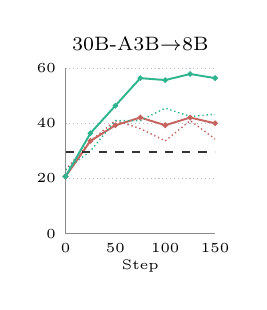
\begin{tikzpicture}
\begin{axis}[
  width=1.9cm, height=2.1cm, scale only axis,
  xmin=0, xmax=150, ymin=0, ymax=60, xtick={0,50,100,150},  xlabel={Step},
  axis lines*=left, axis line style={black!45}, tick style={draw=none}, ytick pos=left,
  ymajorgrids, grid style={densely dotted, black!25}, every tick label/.append style={font=\tiny},
  ylabel style={font=\tiny, yshift=-3pt}, xlabel style={font=\tiny, yshift=4pt}, title style={font=\scriptsize, yshift=-3pt},
  title={30B-A3B$\to$8B},
]
\addplot[vanRed, line width=0.7pt, mark=*, mark size=0.6pt] coordinates {(0,20.7) (25,33.6) (50,39.3) (75,42.1) (100,39.3) (125,42.1) (150,40.0)};
\addplot[vanRed, densely dotted, line width=0.5pt] coordinates {(0,23.1) (25,33.6) (50,41.0) (75,38.1) (100,33.6) (125,41.0) (150,34.3)};
\addplot[r2sGreen, line width=0.7pt, mark=*, mark size=0.6pt] coordinates {(0,20.7) (25,36.4) (50,46.4) (75,56.4) (100,55.7) (125,57.9) (150,56.4)};
\addplot[r2sGreen, densely dotted, line width=0.5pt] coordinates {(0,23.1) (25,29.9) (50,41.0) (75,41.0) (100,45.5) (125,42.5) (150,43.3)};
\draw[dashed, black!80, line width=0.6pt] (rel axis cs:0,0.4921) -- (rel axis cs:1,0.4921);
\end{axis}
\end{tikzpicture}
\hfill
\\[3pt]
{\tiny \tikz[baseline=-0.4ex]{\draw[vanRed, line width=0.7pt] (0,0.065) -- (0.4,0.065);}\,Vanilla OPD\quad \tikz[baseline=-0.4ex]{\draw[r2sGreen, line width=0.7pt] (0,0.065) -- (0.4,0.065);}\,\method{}\quad Solid: seen / canonical\quad Dotted: unseen / pool\quad \tikz[baseline=-0.4ex]{\draw[dashed, black!80, line width=0.6pt] (0,0.065) -- (0.4,0.065);}\,Teacher Alone}
\caption{\textbf{Success over training in every cell of \Cref{tab:main}.} Vanilla and \method{} students, one decode every 25 updates (update 0: untrained). Solid: seen split or WebShop's canonical goals; dotted: unseen split or its 256-goal pool; dashed: the teacher acting alone on the seen split.}
\label{fig:curves-all}
\end{figure}
